\clearpage
\section{Diffusion Distance}

The diffusion distance is given by $\sqrt{Dt}$, which is found in the equation that is used to describe the concentration after a time $t$ in a thin layer of the diffusing species is concentrated at $x=0$ of a semi-infinte sample \cite{diff}:
\begin{align}
  \label{eq:3}
  c(x,t)&=\dfrac{M}{\sqrt{\pi D t} \exp\left(-\dfrac{x^2}{4DT}\right)}.
\end{align}

Using the previous statement, the difussion distance was calculated using a time range from zero to (tengo que arreglar esta parte, porque creo que meti la pata con el calculo del tiempo :c). The plots for the diffusion distance as a function of time and the lilnealization of the diffusion distance are shown in the figure \ref{fig:length}.

\subsection{Self-diffusion}

The shoshfdos

\begin{figure}[h]
 \centering
 \captionsetup{justification=centering}
  \subfloat[]{
   \label{fig:d}
    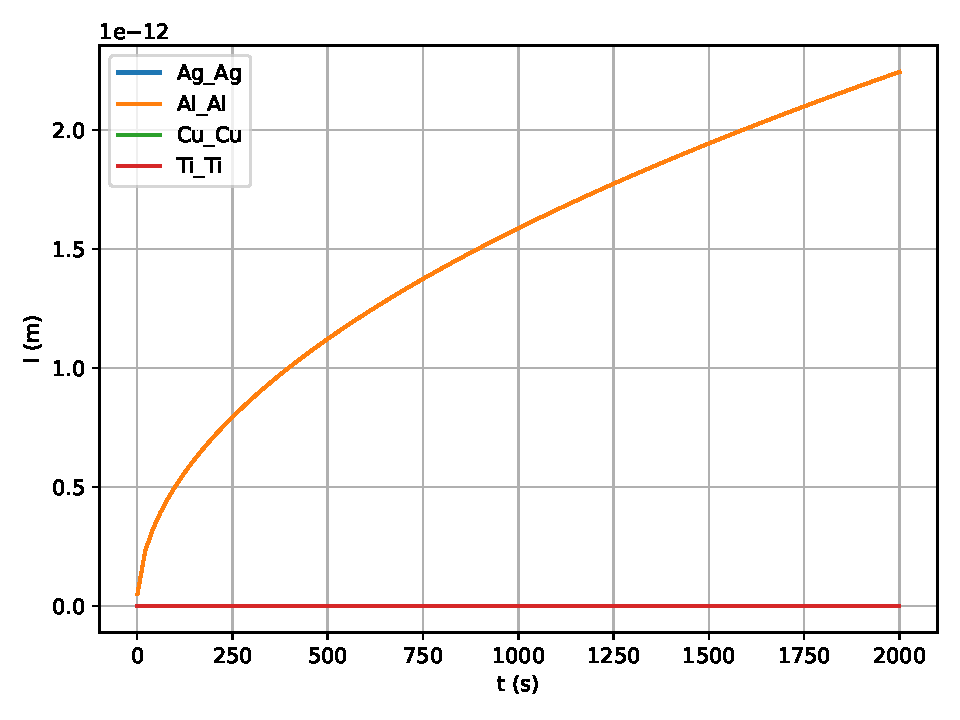
\includegraphics[width=0.5\textwidth]{graficas/l_self.pdf}}
  \subfloat[]{
   \label{fig:lnd}
    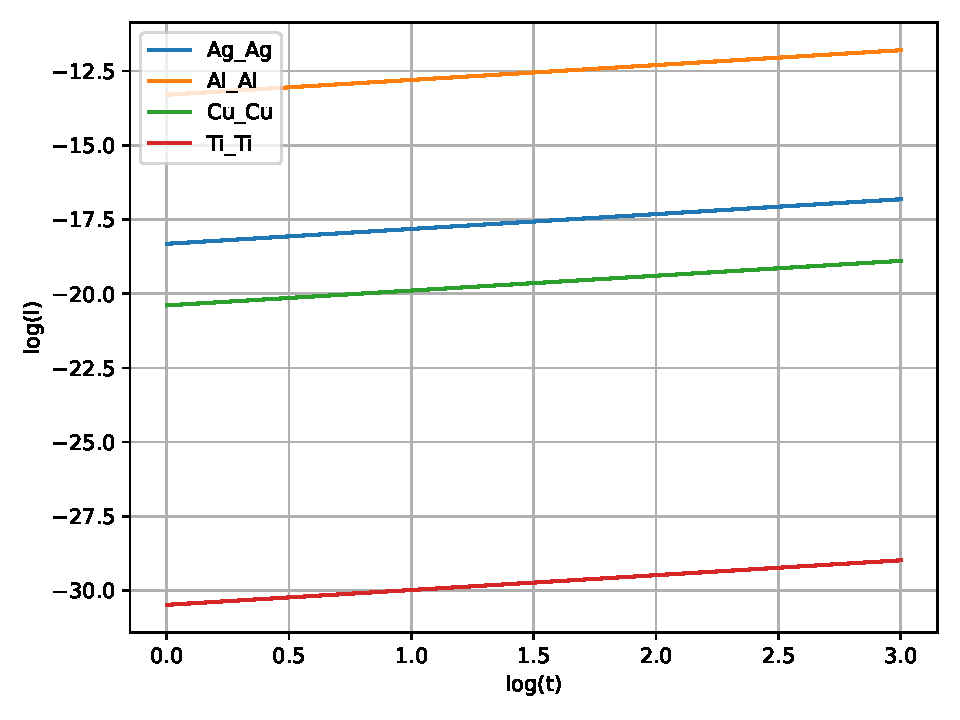
\includegraphics[width=0.5\textwidth]{graficas/log(l)_self.pdf}}
 \caption{a) Diffusion coefficient $D$ ($m^2/s)$ as a function of temperature $T$ (K) and b) logarithm of the diffusion coefficient $ln(D)$ as a function of the inverse of temperature $1/T$ ($K^{-1}$). \\
 \textit{Source: Data from \citep{kakusan}, visualization by the author (code available at \citep{mygit}).}}
 \label{fig:diffusion}
\end{figure}


\subsection{Solute diffusion}

The fsdfojsofdjsodfs

\begin{figure}[h]
 \centering
 \captionsetup{justification=centering}
  \subfloat[]{
   \label{fig:d}
    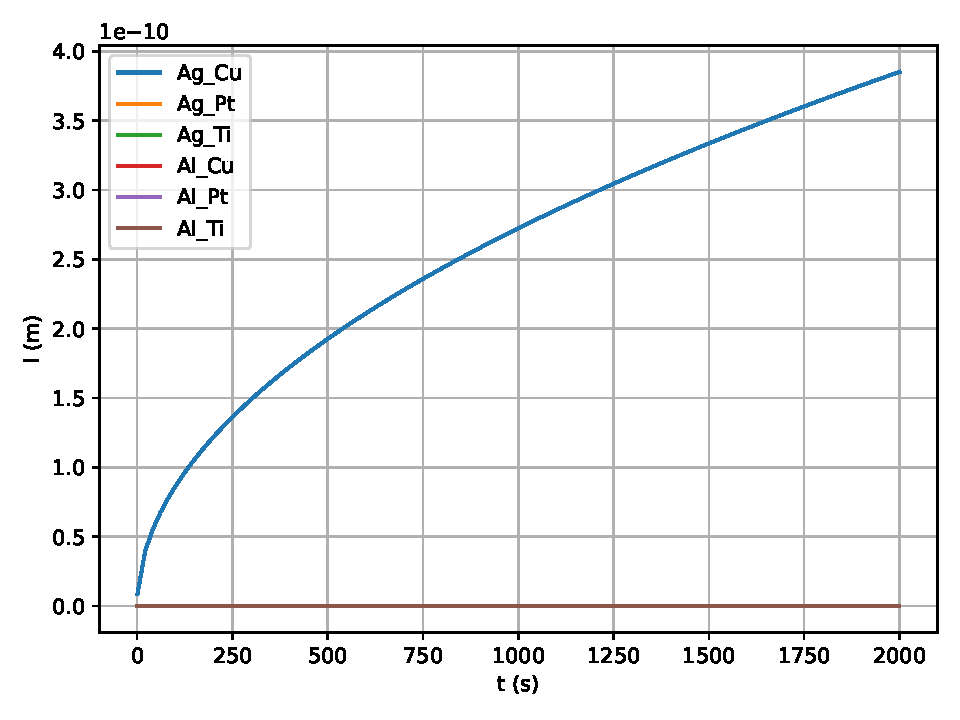
\includegraphics[width=0.5\textwidth]{graficas/l_other.pdf}}
  \subfloat[]{
   \label{fig:lnd}
    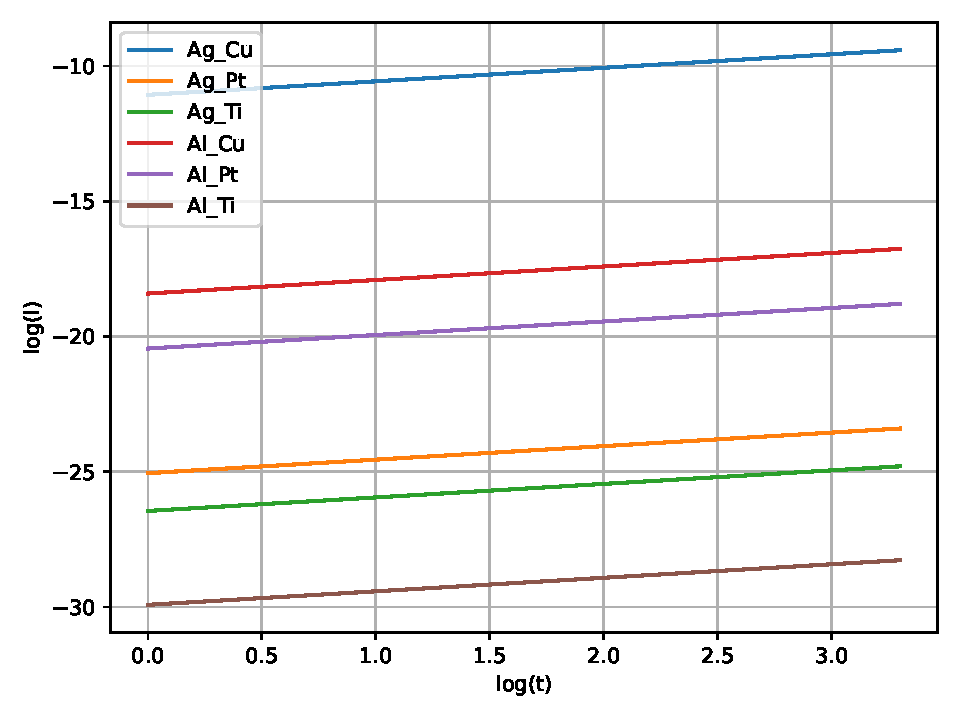
\includegraphics[width=0.5\textwidth]{graficas/log(l)_other.pdf}}
 \caption{a) Diffusion coefficient $D$ ($m^2/s)$ as a function of temperature $T$ (K) and b) logarithm of the diffusion coefficient $ln(D)$ as a function of the inverse of temperature $1/T$ ($K^{-1}$). \\
 \textit{Source: Data from \citep{kakusan}, visualization by the author (code available at \citep{mygit}).}}
 \label{fig:diffusion}
\end{figure}
